\documentclass{beamer}

\usepackage{eecs}

\usepackage[all]{xy}
\usepackage{xmpmulti}
\usepackage{pdfpages}
\usepackage{fancyvrb}

\SaveVerb{bind}+>>=+
\SaveVerb{from}+<-+

\title[EECS 700]{EECS 700\\Functional Programming}
\author[Andy Gill]{Dr. Andy Gill}
\institute{University of Kansas}
\date{October 19, 2012}

\begin{document}

\frame{\titlepage}

\begin{frame}[fragile]
\frametitle{Blank Canvas}
\Large
\begin{itemize}
\item New library for simple graphics
\item Uses HTML5's \verb|<canvas>| capabilities as viewport
\item Javascript examples can be transliterated into Haskell    
\item Fast enough for basic animations
\end{itemize}
\begin{columns}
\begin{column}{0.45\textwidth}
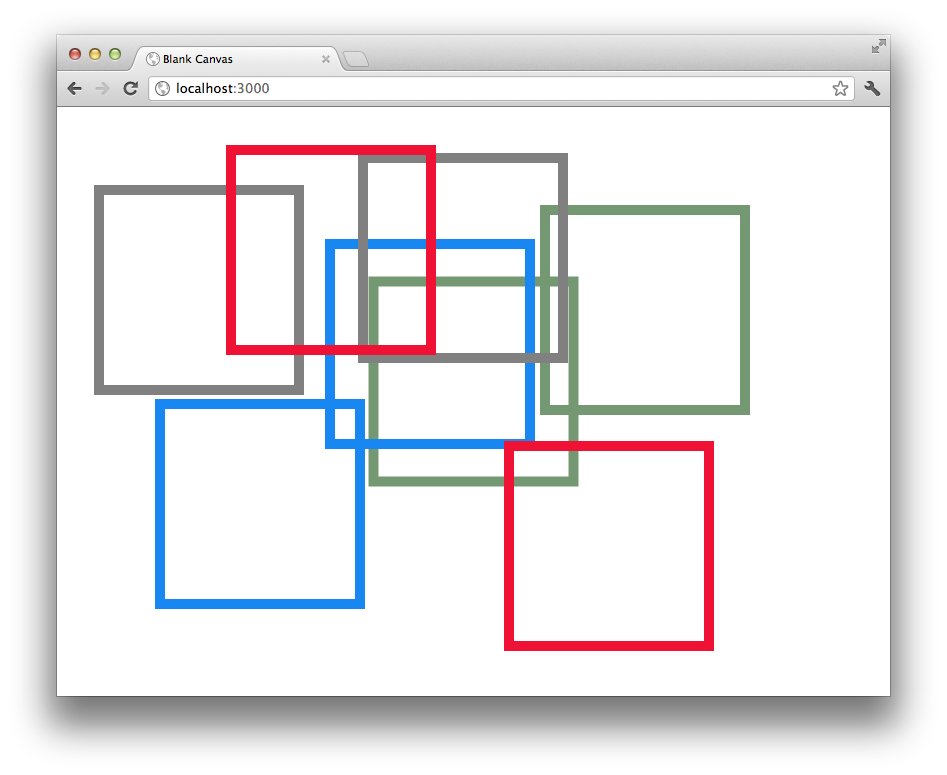
\includegraphics[width=150pt]{squares.png}
\end{column}
\begin{column}{0.55\textwidth}
\begin{codeblock}[0.6]
\footnotesize
\begin{verbatim}
...
translate (x,y)
beginPath()
moveTo(-100,-100)
lineTo(-100,100)
lineTo(100,100)
lineTo(100,-100)
closePath()
lineWidth 10
strokeStyle color
stroke()
...
\end{verbatim}
\end{codeblock}
\end{column}
\end{columns}
%\frameskip{}
%Why another image processing tool?
%\begin{itemize}
%\item Need a machine independent way of scripting up graphics in Haskell.
%\end{itemize}


\end{frame}

\begin{frame}[fragile]
\frametitle{This class: Design and Implementation of blank-canvas}
\Large
\begin{itemize}
\item How to structure small examples
\item How to transliterate from Javascript tutorials
\item Animation and Interaction
\item Design and Implementation of the the Canvas DSL
\item Extended Example: tic-tac-toe
\frameskip{}
\item blank-canvas is available on hackage (real soon now)
\end{itemize}
\begin{execblock}[0.65]
\begin{verbatim}
 % cabal install blank-canvas
\end{verbatim}
\end{execblock}
\begin{itemize}
\item Also on github: {\tt\small https://github.com/andygill/blank-canvas}
\end{itemize}
\end{frame}

\begin{frame}[fragile]
\frametitle{First Example: red line}
\Large



\begin{columns}
\begin{column}{0.40\textwidth}
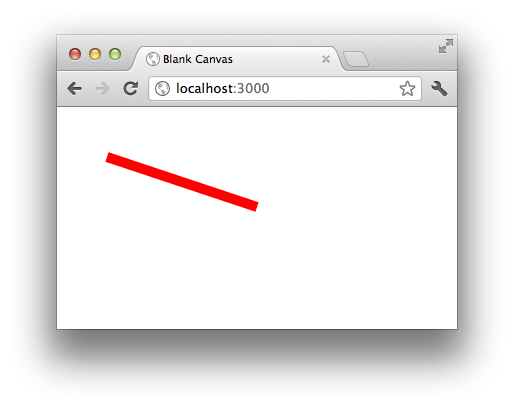
\includegraphics[width=150pt]{red-line.png}
\end{column}
\begin{column}{0.60\textwidth}
\begin{codeblock}[0.95]
\footnotesize
\begin{semiverbatim}
import Graphics.Blank
\uncover<2->{
main = blankCanvas 3000 \$ \\ context -> do\uncover<3->{
        send context \$ do\uncover<4->{
                moveTo(50,50)
                lineTo(200,100)
                lineWidth 10
                strokeStyle "red"
                stroke}}}
\end{semiverbatim}
\end{codeblock}
\end{column}
\end{columns}

\frameskip{}
\only<1>%
{First, include the {\tt Graphics.Blank} module.}
\only<2>%
{Second, main calls {\tt blankCanvas}, with two arguments:%
\begin{itemize}
\item The port (3000) to publish the application on; and
\item and what to do with canvas.
\end{itemize}
}
\only<3>%
{Third, we {\tt send} to the canvas a list of monadic commands}
\only<4>%
{Finally, here are the commands to draw a {\color{red}red} line}

\end{frame}

\begin{frame}[fragile]
\frametitle{Architecture of {\tt blank-canvas}}
\Large


\begin{tabular}{ccc}
Haskell & &\\
\begin{minipage}[b]{.3\textwidth}
\begin{codeblock}[0.85]
\small
Your application:
\footnotesize ``please draw red line''
\end{codeblock}
\begin{codeblock*}[0.85]{{\tt blank-canvas}}
\tiny
Canvas commands for drawing pictures.
\end{codeblock*}
\begin{codeblock*}[0.85]{{\tt scotty}}
\tiny 
Support for RESTful APIs.
\end{codeblock*}
\begin{codeblock*}[0.85]{{\tt warp}}
\tiny
Receiving web requests from clients;
give back responses \& web pages.
\end{codeblock*}
\end{minipage}
    & ~~~$\Huge\Longleftrightarrow$ & \raisebox{-.3\height}{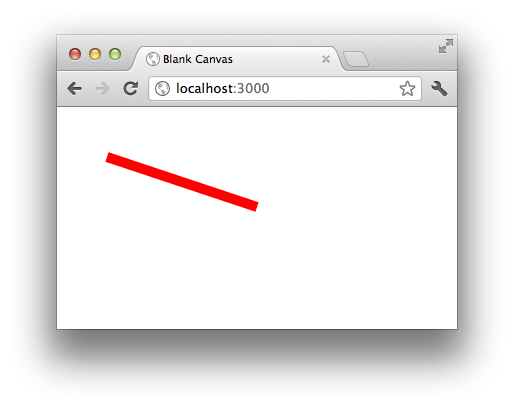
\includegraphics[width=150pt]{red-line.png}}\\
Software Stack & & Web Browser\\
\end{tabular}


\end{frame}

\begin{frame}[fragile]
\frametitle{Types in blank-canvas}
\large
\begin{codeblock}[0.99]
\begin{semiverbatim}
-- Create a web server. Run the given function with
-- a fresh Context each time our webpage is called.
blankCanvas :: Int -> (Context -> IO ()) -> IO ()

-- Sends a set of Canvas commands to the canvas. 
-- Attempts to common up as many commands as possible. 
-- A canvas command *may* return a result, which
-- will get passed back from the browser to the 
-- user, via the IO a.
send :: Context -> Canvas a -> IO a

-- Example of Canvas command
moveTo :: (Float, Float) -> Canvas ()
\end{semiverbatim}
\end{codeblock}        
\end{frame}




\begin{frame}[fragile]
\frametitle{Flow of Types}

\large
\begin{tabular}{rcrr}
        & \multicolumn{2}{c}{~~~~~{\tt Canvas a}}\\
        & \multicolumn{2}{c}{~~~~$\downarrow$}                    & Your Application\\
{\tt send ::}& \multicolumn{2}{c}{{\tt Context -> Canvas a -> IO a}}\\
        \cline{2-3}\noalign{\smallskip}
        & {\tt Context}~$\uparrow$      & $\downarrow$~{\tt IO~()}    & ~~~~{\tt  blank-canvas}\\
        \cline{2-3}\noalign{\smallskip}
        & \multicolumn{2}{c}{\tt IO ()}                                   & {\tt scotty}\\
\end{tabular}

\frameskip
\frameskip
\frameskip

\begin{itemize}
\item Drawings are constructed using the {\tt Canvas} monad
\item {\tt send} pushes a Canvas drawing to the screen
\item No way to get from inside the {\tt Canvas} monad
to the {\tt IO} monad
\item Hence, programs are written in {\tt IO}, with
islands of {\tt Canvas} drawing rendered via {\tt send}.
\item {\tt Canvas} results are returned to {\tt IO} via {\tt send}.
\end{itemize}        

\end{frame}



\begin{frame}[fragile]
\frametitle{From: {\tt http://www.html5canvastutorials.com/}}

\begin{codeblock}[0.8]
\tiny
\begin{semiverbatim}
<!DOCTYPE HTML>
<html>
  <head>
    <style>
      body \{
        margin: 0px;
        padding: 0px;
      \}
      #myCanvas \{
        border: 1px solid #9C9898;
      \}
    </style>
    <script>
      window.onload = function() \{
        var canvas = document.getElementById("myCanvas");
        var context = canvas.getContext("2d");

        \alert{context.moveTo(100, 150);
        context.lineTo(450, 50);
        context.stroke();}
      \};

    </script>
  </head>
  <body>
    <canvas id="myCanvas" width="578" height="200"></canvas>
  </body>
</html>
\end{semiverbatim}
\end{codeblock}
\end{frame}

\begin{frame}[fragile]
\frametitle{Example of Javascript to Haskell Transliteration}

\begin{columns}
\begin{column}{0.50\textwidth}
\begin{codeblock*}[0.85]{Javascript}
\begin{verbatim}
context.moveTo(100, 150);
context.lineTo(450, 50);
context.stroke();
\end{verbatim}
\end{codeblock*}
\end{column}

\pause{}
\begin{column}{0.50\textwidth}
\begin{codeblock*}[0.65]{Haskell}
\begin{verbatim}
send context $ do
   moveTo(100, 150)
   lineTo(450, 50)
   stroke()
\end{verbatim}
\end{codeblock*}
\end{column}

\end{columns}

\frameskip
\frameskip
\frameskip

\pause{}

\centering
\begin{codeblock*}[0.6]{Types in {\tt blank-canvas}}
\begin{verbatim}
moveTo :: (Float,Float) -> Canvas ()
lineTo :: (Float,Float) -> Canvas ()
stroke :: ()            -> Canvas ()

send :: Context -> Canvas a -> IO a
\end{verbatim}
\end{codeblock*}

\end{frame}        
        
\begin{frame}[fragile]
\frametitle{Supported Canvas Commands}

\begin{codeblock}[0.6]
\tiny
\begin{verbatim}
arc :: (Float,Float,Float,Float,Float,Bool) -> Canvas ()
beginPath :: () -> Canvas ()
clearRect :: (Float,Float,Float,Float) -> Canvas ()
closePath :: () -> Canvas ()
fill :: () -> Canvas ()
fillStyle :: String -> Canvas ()
fillText :: (String,Float,Float) -> Canvas ()
font :: String -> Canvas ()
lineCap :: String -> Canvas ()
lineTo :: (Float,Float) -> Canvas ()
lineWidth :: Float -> Canvas ()
miterLimit :: Float -> Canvas ()
moveTo :: (Float,Float) -> Canvas ()
restore :: () -> Canvas ()
rotate :: Float -> Canvas ()
scale :: (Float,Float) -> Canvas ()
save :: () -> Canvas ()
stroke :: () -> Canvas ()
strokeText :: (String,Float,Float) -> Canvas ()
strokeStyle :: String -> Canvas ()
textAlign :: String -> Canvas ()
textBaseline :: String -> Canvas ()
transform :: (Float,Float,Float,Float,Float,Float) -> Canvas ()
translate :: (Float,Float) -> Canvas ()        
\end{verbatim}        
\end{codeblock}
\end{frame}

\begin{frame}[fragile]
\frametitle{Animation}

\Large
Animation is simply a matter of sending draw commands fast enough to the
browser window.

\begin{codeblock}[0.9]
\footnotesize
\begin{verbatim}
module Main where

import Graphics.Blank

main = blankCanvas 3000 $ \ context -> loop context (0 :: Float)

loop context n = do
        send context $ do
                -- clear the canvas
                ...
                -- draw the square
                ...
                
        loop context (n + 0.01)
\end{verbatim}
\end{codeblock}

\end{frame}

\begin{frame}[fragile]
\frametitle{Rotating Square}

\begin{columns}
\begin{column}{0.40\textwidth}
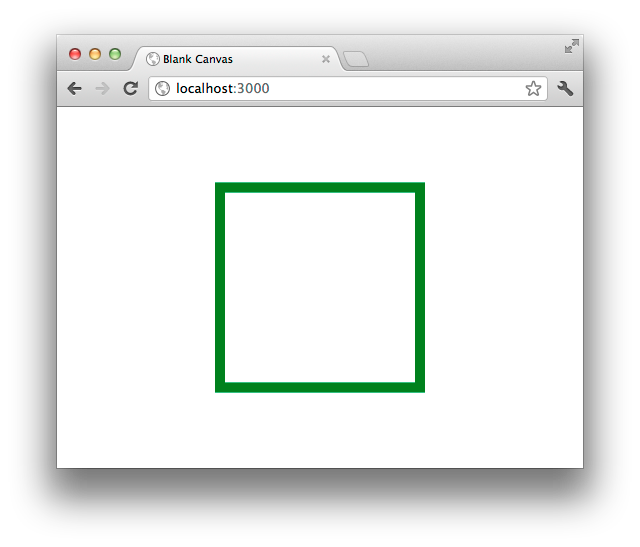
\includegraphics[trim = 25mm 30mm 25mm 25mm, clip, width=90pt]{1.png}\\
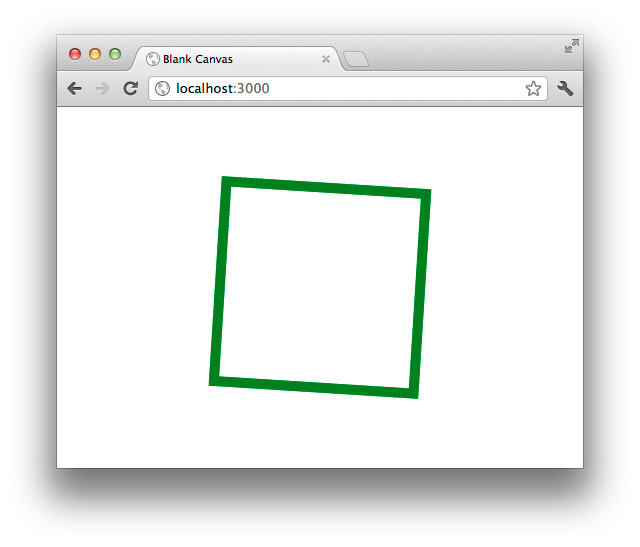
\includegraphics[trim = 25mm 30mm 25mm 25mm, clip, width=90pt]{3.png}\\
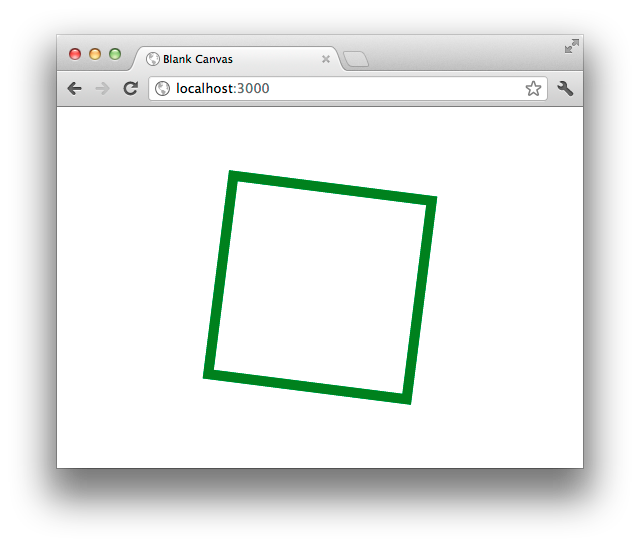
\includegraphics[trim = 25mm 30mm 25mm 25mm, clip, width=90pt]{5.png}
\end{column}
\begin{column}{0.60\textwidth}
\begin{codeblock}[0.95]
\footnotesize
\begin{semiverbatim}
loop context n = do
    send context \$ do
        (width,height) <- size
        clearRect (0,0,width,height)
        beginPath()
        save()
        translate (width / 2,height / 2)
        rotate (pi * n)
        beginPath()
        moveTo(-100,-100)
        lineTo(-100,100)
        lineTo(100,100)
        lineTo(100,-100)
        closePath()
        lineWidth 10
        strokeStyle "green"
        stroke()
        restore()
    loop context (n + 0.01)
\end{semiverbatim}
\end{codeblock}
\end{column}
\end{columns}


\end{frame}


\begin{frame}[fragile]
\frametitle{Explaining the drawing of the square}

\tiny

\begin{columns}[t]
\begin{column}{0.5\textwidth}

\begin{codeblock}[0.8]
\begin{semiverbatim}
(width,height) <- size
clearRect (0,0,width,height)
beginPath()
\end{semiverbatim}
\end{codeblock}

\begin{codeblock}[0.8]
\begin{semiverbatim}
save()
\end{semiverbatim}
\end{codeblock}

\begin{codeblock}[0.8]
\begin{semiverbatim}
translate (width / 2,height / 2)
rotate (pi * n)
\end{semiverbatim}
\end{codeblock}

\begin{codeblock}[0.8]
\begin{semiverbatim}
beginPath()
moveTo(-100,-100)
lineTo(-100,100)
lineTo(100,100)
lineTo(100,-100)
closePath()
lineWidth 10
strokeStyle "green"
stroke()
\end{semiverbatim}
\end{codeblock}

\begin{codeblock}[0.8]
\begin{semiverbatim}
restore()
\end{semiverbatim}
\end{codeblock}

\end{column}
\begin{column}{0.4\textwidth}

\vskip 10pt
\noindent
Clear the screen.\\
({\tt beginPath()} is needed for line drawings.)

\vskip 25pt
\noindent
Save the state of the canvas. This is good practice.


\vskip 20pt
\noindent
These translations are applied to all coordinates.

\vskip 25pt
\noindent
At last we can draw the square!  Notice how we draw
a 200x200 square, centered on (0,0), 
and rely on the previous translations
to give us rotation.

\vskip 55pt
\noindent
Restore the state of the canvas.\\
This undoes the translations.

\end{column}
\end{columns} 
\end{frame}

\begin{frame}[fragile]
\frametitle{Interaction}

\begin{itemize}
\item The browser can send your Haskell program {\em events\/}.
\item Example of events are \verb|MouseDown|, \verb|MouseMove|, and \verb|KeyPress|.
\item {\bf You can wait for specific events using the {\tt Canvas} monad.}
\end{itemize}

\begin{codeblock*}[0.9]{Handling Events}
\begin{verbatim}
data Event = Event
           { jsCode  :: Int  -- event specific code
           , jsMouse :: Maybe (Int,Int)
           }

readEvent    :: EventName -> Canvas Event
tryReadEvent :: EventName -> Canvas (Maybe Event)
flushEvents  :: EventName -> Canvas ()
\end{verbatim}
\end{codeblock*}

\frameskip{}
\frameskip{}
Using {\tt Canvas\/}, you are always examining one type of event at a time.
\end{frame}

\begin{frame}[fragile]
\frametitle{[Advanced Aside] Interaction with multiple {\tt EventName}s}

\begin{itemize}
\item You can also directly handle events yourself.
\end{itemize}
\begin{codeblock}
\begin{verbatim}
events :: Context -> EventName -> IO EventQueue
\end{verbatim}
\end{codeblock}

\begin{itemize}
\item Event queues use Software Transactional Memory, allowing for
multiple types of events to be waited for at the same time.
\end{itemize}
\begin{codeblock}
\begin{verbatim}
type EventQueue = TChan Event
\end{verbatim}
\end{codeblock}

\frameskip{}
\begin{itemize}
\item The {\tt Canvas} interactions are built on top of this API.
\end{itemize}



\end{frame}

\begin{frame}[fragile]
\frametitle{Squares placed using the mouse}

\begin{codeblock}[0.8]
\tiny
\begin{semiverbatim}
main = blankCanvas 3000 \$ \\ context -> do
          let loop (x,y) (color:colors) = do
                send context \$ do
                        save()
                        translate (x,y)
                        beginPath()
                        moveTo(-100,-100)
                        lineTo(-100,100)
                        lineTo(100,100)
                        lineTo(100,-100)
                        closePath()
                        lineWidth 10
                        strokeStyle color
                        stroke()
                        restore()
\alert{
                event <- send context \$ readEvent MouseDown
                case jsMouse event of
                        Nothing -> loop (x,y) colors
                        Just (x',y') -> loop (fromIntegral x',fromIntegral y') colors
}
          (width,height) <- send context size

          loop (width / 2,height / 2)
               (cycle [ "#749871", "#1887f2", "#808080", "f01234"])
\end{semiverbatim}
\end{codeblock}
\end{frame}

\begin{frame}[fragile]
\frametitle{blank-canvas DSL}

Main data structures in {\tt blank-canvas} are: 
\begin{itemize}
\item {\tt Canvas}      -- Monad, inside IO via {\tt send}.
\item {\tt Context}     -- handle for a specific browser's viewport.
\item {\tt Event}       -- Something happens.
\item {\tt EventName}   -- Names for possible interactions from user.
\item {\tt EventQueue}  -- Place to store events until they are read.
\end{itemize}
\
\frameskip{}
Interesting part is the {\tt Canvas} monad. 
\begin{itemize}
\item Is {\tt Canvas} shallow or deep?
\end{itemize}

\end{frame}

\begin{frame}[fragile]
\frametitle{The Canvas Monad}

{\tt Canvas} provides a deep DSL. This allows for certain optimizations,
specifically we try bundle together as much as possible when
sending drawing commands to the browser.

\begin{codeblock}
\tiny
\begin{verbatim}
data Canvas :: * -> * where
        Command :: Command                           -> Canvas ()
        Bind    :: Canvas a -> (a -> Canvas b)       -> Canvas b
        Return  :: a                                 -> Canvas a
        Get     :: EventName -> (EventQueue -> IO a) -> Canvas a
        Size    ::                                      Canvas (Float,Float)

instance Monad Canvas where
        return = Return
        (>>=) = Bind

data Command
        = Arc (Float,Float,Float,Float,Float,Bool)
        | BeginPath
        | ClearRect (Float,Float,Float,Float)
        | ClosePath
        | Fill
        ....
\end{verbatim}

\end{codeblock}

\end{frame}

\begin{frame}[fragile]
\frametitle{The Canvas Commands}

There is a {\tt Canvas} command for each Javascript function.

\begin{codeblock}[0.6]
\tiny
\begin{verbatim}
...
fill :: () -> Canvas ()
fill () = Command Fill

fillStyle :: String -> Canvas ()
fillStyle = Command . FillStyle

fillText :: (String,Float,Float) -> Canvas ()
fillText = Command . FillText

font :: String -> Canvas ()
font = Command . Font
...
\end{verbatim}
\end{codeblock}

\frameskip
These are auto-generated from a table.

\frameskip
Some Javascript commands use assignment; we use function arguments.

\begin{columns}
\begin{column}{0.50\textwidth}
\begin{codeblock*}[0.80]{Javascript}
\footnotesize
\begin{semiverbatim}
context.font \alert{=} "30pt Calibri"
\end{semiverbatim}
\end{codeblock*}
\end{column}

\begin{column}{0.50\textwidth}
\begin{codeblock*}[0.52]{Haskell}
\footnotesize
\begin{verbatim}
font "30pt Calibri"
\end{verbatim}
\end{codeblock*}
\end{column}

\end{columns}

\end{frame}

\begin{frame}[fragile]
\frametitle{The Canvas Commands}

There is a {\tt Canvas} command for each Javascript function.

\begin{codeblock}[1]
\tiny
\begin{verbatim}
instance Show Command where
  ...
  show Fill = "c.fill();"
  show (FillStyle (a1)) = "c.fillStyle = (" ++ show a1 ++ ");"
  show (FillText (a1,a2,a3)) = "c.fillText(" ++ show a1 ++ "," ++ showJ a2 ++ "," ++ showJ a3 ++ ");"
  show (Font (a1)) = "c.font = (" ++ show a1 ++ ");"
  ...
\end{verbatim}
\end{codeblock}

\frameskip
{\tt send} works by calling {\tt show} on all the commands, and sending them to the browser
in a single combined javascript script.
\end{frame}

\begin{frame}[fragile]
\frametitle{The Canvas Webserver}

We use the {\tt scotty} web service provider. This make the handling 
of web page issues straightforward.

\begin{codeblock}[0.6]
\tiny
\begin{semiverbatim}
blankCanvas :: Int -> (Context -> IO ()) -> IO ()
blankCanvas port actions = do
   ...
   app <- scottyApp $ do
        ...

        get "/" $ file $ dataDir ++ "/static/index.html"
        
        post "/start" $ do
            ... \alert{create a new context} ...

        post "/event/:num" $ do
             ... \alert{add an event onto the correct queue} ...

        get "/canvas/:num" $ do
            ... \alert{wait for the user to send commands} ...
            ... (in textual / javascript form) ...

   run port app
\end{semiverbatim}
\end{codeblock}

\end{frame}

\begin{frame}[fragile]
\frametitle{Tic-Tac-Toe}

\centering
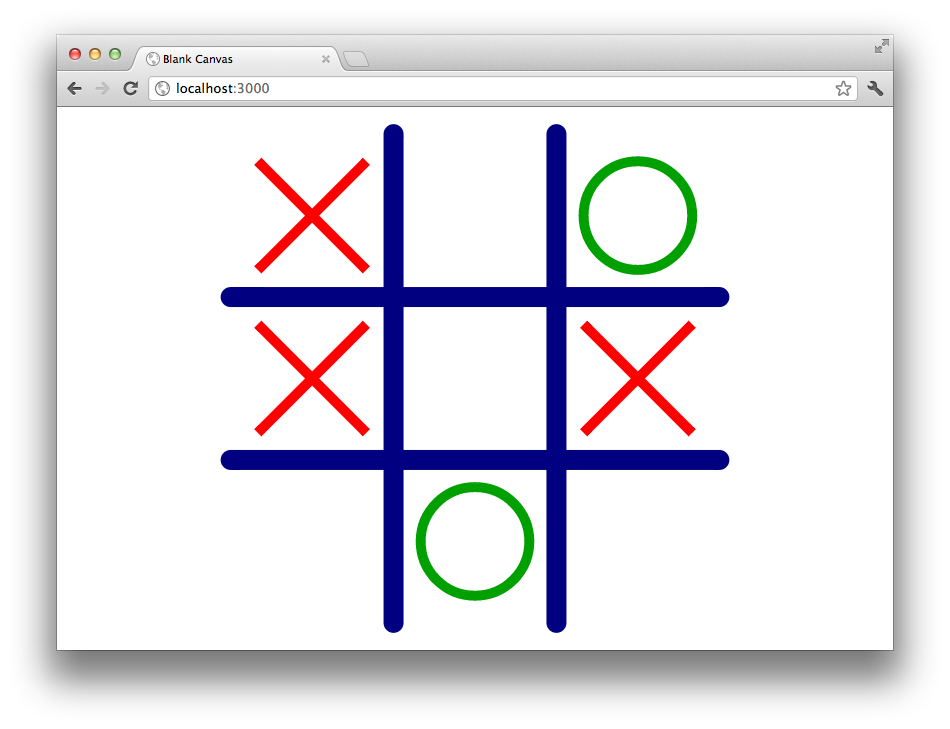
\includegraphics[width=290pt]{xox.png}


\end{frame}

\end{document}
